\documentclass{article}

\usepackage{listings, lstautogobble}
\lstset{
	autogobble=true,
	aboveskip=20pt,
	belowskip=20pt,
	showstringspaces=false
}
\usepackage{graphicx}
\usepackage{hyperref}
\hypersetup{colorlinks=true, linkcolor=black, linktoc=all, urlcolor=blue, pdfnewwindow=true}
\usepackage{url}

\usepackage[utf8]{inputenc}
\inputencoding{utf8}

\usepackage{titling}

\pretitle{%
	\begin{center}
	\LARGE
	\hspace*{18mm}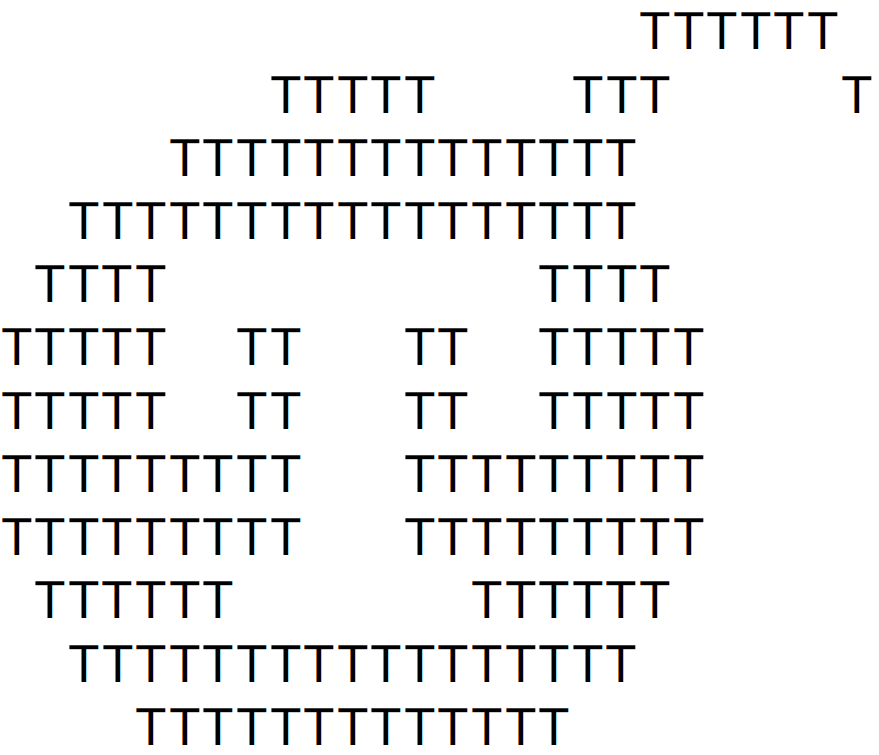
\includegraphics[width=90mm]{logo.png}\\[\bigskipamount]
}
\posttitle{\end{center}}

\title{Turbo-Bomber}
\date{January 06, 2016}
\author{Tim Gevers, Jonas Krug, Hendrik Sieck}

\begin{document}
	\pagenumbering{gobble}
	\maketitle
	\newpage
	
	\tableofcontents
	\newpage
	
	\pagenumbering{arabic}
	
	\section{Specification}
		The main goal is to implement a game like ``Bomberman''. The player plays in a quadratic world and tries to clear its way with clever placed bombs. Some walls contain items that increase several properties of the player and its utilities.
		
		\subsection{Criteria for evaluation}
			\subsubsection{Read from files}
				The game uses files to be configurable and modifiable.
			
			\subsubsection{Random item drops}
				When a tile is destroyed by a player it is possible that the wall drops an item. An algorithm chooses based on probabilties which item is then dropped. The items are generally \emph{Power Ups}.
			
			\subsubsection{Read keys from the keyboard}
				For a fast game keyboard input is required. The input is taken directly without any buffering. (Does also not require pressing the Return-key.)
			
			\subsubsection{Move player}
				The player is able to walk around in the map to place bombs.
			
			\subsubsection{Animations}
				The game will be outputted to the command line via a common used library called \emph{ncurses}. This includes also animations and a simple text based user interface.
			
			\subsubsection{Place bombs}
				Bombs can be placed on empty tiles of the map. They have simple detonation physics which gives them the ability to destroy walls and harm players.
			
			\subsubsection{Destructable map}
				The map consists of several destructable walls which may be destroyed by bombs. When these walls are destroyed they may drop an item.
			
			\subsubsection{Game loop}
				To be able to interact with the player inputs and play animations the game has a main loop. This main loop will process several events (e.g. keypresses) and actions.
	
	\section{Design}
		\subsection{Structure of the game}
			The game has a main information stream. This stream starts at the user. The user provides informations to the program which are especially keyboard inputs. These keyboard events are processed and moved to the \emph{gameplay}-module. This module is the central module which consists of the complete game logic. The \emph{gameplay}-module generates a data structure that is consumed by the \emph{graphics}-module. A framebuffer (of the \emph{ncurses}-library) is then filled by the \emph{graphics}-module. The module also frequently updates the framebuffer to produce some animations. \\
			
			The complete information stream is processed each frame. As a result each frame keyboard events are processed, the game logic (\emph{gameplay}-module) reacts to this events and the \emph{graphics}-module displays the game on the screen.
		
		\subsection{Important data structures}
			\subsubsection{Properties of a map tile}
				\begin{itemize}
					\item type of the tile (wall, destructable wall, floor)
					\item player that stands on the tile
					\item explosion animation informations
					\item bomb that is placed on the tile
					\item random generated item (\emph{Power Ups}) of the tile
					\item timing informations for items and explosions
				\end{itemize}
			
			\subsubsection{Properties of a player}
				\begin{itemize}
					\item health points
					\item movement cooldown (to decrease movement speed)
					\item position on the map
					\item amount of placeable bombs
					\item amount of currently placed bombs
					\item current item
					\item item usage timing (duration, used time) (some items are limited in time)
				\end{itemize}
	
	\section{Conventions}
		\subsection{Coding style}
			Use \emph{Allman}-style with the following changes:
			\begin{itemize}
				\item Do not write whitespaces after \emph{while}, \emph{if} or other control statements.
				\item Do use tabulators as indentation.
				\item Do not use single line statements (e.g. in \emph{while}, \emph{if}). Always use (curly) brackets around these statements.
			\end{itemize}
		
		\subsection{Nomenclature/Naming}
			\subsubsection{Functions}
				Names of a function in the code should have the following nomenclature:
				
				\begin{lstlisting}
					<module name>_<part of the module>_<action to perform>();
				\end{lstlisting}
				
				\paragraph{module name} Each module consists of one source file. It has the name of the module. If the module has multiple words the words are separated by ``-''-characters, in the function name ``\_''-characters. An example file name would be: ``image-loader.c''. An example function name can be found in the \emph{action to perform}-paragraph.
				
				\paragraph{part of the module} A module can be splitted into multiple parts. The parts are summarized in a single module file. If a part has multiple words the words are separated by ``\_''-characters. An example function name can be found in the next paragraph. The part can be omitted if the module only has one part.
				
				\paragraph{action to perform} The action describes what a function will do with the part in the module. If the action has multiple words the words are separated by characters. An example function name would be: ``image\_loader\_file\_informations\_print();''.
			
			\subsubsection{Variables}
				Do not use global variables. Variables needed in a module can be declared as ``static''-variables at the head of the source file. Variables should always be initialized with a default value (at compile time). Variables have the following nomenclature:
				
				\begin{lstlisting}
					static int <module name>_<part of the module>_<property name> = 0;
				\end{lstlisting}
				
				\emph{module name} and \emph{part of the module} are described ahead.
				
				\paragraph{property name} The property which the variable holds the value for. If the property name has multiple words the words are separated by characters. An example function name would be: ``static int image\_loader\_file\_informations\_count = 0;''.
		
		\subsection{Other}
			\begin{enumerate}
				\item Do not upload binaries.
				\item Do describe the commits usefully.
				\item Do not commit multiple features in one commit. Split them into several commits.
				\item Do not use special characters (whitespaces included):
					\begin{itemize}
						\item Do not use special characters in the program (code).
						\item Do not use special characters in directory names.
						\item Do not use special characters in file names.
						\item Do not use special characters in commit descriptions.
					\end{itemize}
				\item Do use English as general language.
				\item Do always document functions. Use the Doxygen documentation style. (\url{http://www.stack.nl/~dimitri/doxygen/manual/index.html})
				\item Do document code when the code does not express its meaning itself.
			\end{enumerate}
\end{document}